\chapter{Исследовательская часть}

В данном разделе описано проведённое исследование и представлены его результаты. Также приведены характеристики устройства, на котором проводились замеры.

\section{Технические характеристики устройства}
Технические характеристики устройства, на котором выполнялось исследование \cite{web_item5}:
\begin{itemize}
	\item операционная система $macOS$ $Monterey$ 12.4;
	\item 8 ГБ оперативной памяти;
	\item процессор $Apple$ $M2$ (базовая частота~---~2400 МГц, но поддержка технологии $Turbo$ $Boost$ позволяет достигать частоты в 3500 МГц).
\end{itemize}

\section{Постановка исследования}
Целью исследования является определение зависимости времени генерации изображе­ния сцены, содержащей изображение мыльных пузырей, от количества потоков, выделяемых для выполнения программы. Исследование проводилось для значений количества выделяемых потоков, не превышающих 25, так как уже на этом значении происходит замедление работы алгоритма, в связи с превышением затрат времени на выделение потока максимально возможных для поддержания ускорения работы программы.
Во время проведения исследования устройство было подключено к блоку питания и не нагружено никакими приложениями, кроме встроенных приложений окружения, окружением и системой тестирования. Оптимизации компилятора были отключены.
По результатам исследования составляется сравнительная таблица и строится график зависимости.

\section{Средства исследования}
Время синтеза сцены замерялось с помощью класса $std::chrono::system\_clock$ \cite{web_item16}, который представляет реальное время. В изображениях для исследования растр имеет одинаковое количество пикселов в обоих плоских измерениях, на самом изображении находится один объект-пузырь и 1 источник света.

\section{Результаты исследования}
Результаты замеров времени выполнения (в мс) приведены в таблице \ref{table:time1}. Количество потоков равное нулю означает, что замер проведён для однопоточной реализации, что отличается от столбца, соответствующего одному потоку, так как для последнего подразумевается именно переключение на дополнительный поток. В замерах использовались изображения размером от $128 \times 128$ пикселов до $512 \times 512$ пикселов.

\begin{table}[H]
	\begin{center}
		\caption{\label{table:time1} Таблица времени выполнения программы (мс)}
		\begin{tabular}{
    |S[table-format=4.0]
    |S[table-format=4.3]
    |S[table-format=4.3]
    |S[table-format=4.3]
    |S[table-format=4.3]
    |S[table-format=4.3]
    |S[table-format=4.3]
    |S[table-format=4.3]|
    }
			\hline
			{\specialcell{Размер\\изображения\\(в пикселах)}} & \multicolumn{7}{c|}{Количество потоков}\\ 
			\cline{2-8}
			&   {0}&{1}&{2}&{4}&{8}&{16}&{25}\\ 
		
			\hline
			128 & 1199.96 & 1202.21 & 610.509 & 329.765 & 215.551 & 200.37 & 213.304 \\ \hline
			256 & 4910.94 & 4916.96 & 2425.05 & 1337.52 & 1074.85 & 983.585  & 995.868 \\ \hline
			384 & 10805.7 & 10808.8 & 5432.39 & 3160.25 & 2498.38 & 2431.28 & 2633.66\\ \hline
			512 & 17347 & 17414.2 & 9592.75 & 5332.85 & 3932.14 & 3802.21 & 3807.14\\ \hline
			
		\end{tabular}
	\end{center}
\end{table}

На рисунке \ref{img:graph1} приведён график, отображающие зависимость времени работы программы от количества выделяемых потоков.

\noindent
\begin{table}[h!]
  \centering
  \begin{tabular}{p{1\linewidth}}
    \centering
    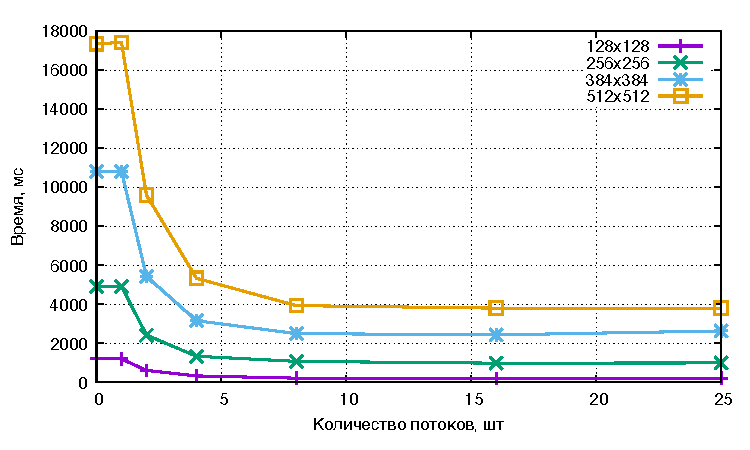
\includegraphics[width=0.65\linewidth]{../images/time.pdf}
    \captionof{figure}{Зависимость времени работы программы от количества выделяемых потоков}
    \label{img:graph1}
  \end{tabular}
\end{table}

\section{Выводы по исследовательской части}
В данном разделе было описано проведённое исследование и представлены его результаты. Также были приведены характеристики устройства, на котором проводилось исследование. Результаты исследования показывают, что наибольшая эффективность достигается при использовании потоков, количество которых не более чем в 2 раза превышает количество ядер процессора. При большем количестве потоков скорость работы программы снижается. Это связано с тем, что программа содержит участки кода, которые выполняются последовательно, поэтому к ним неприменимо распараллеливание. Тогда определённая доля суммарного времени выполнения всегда будет оставаться постоянной и ускорение достигнет своего предела. Данный вывод согласуется с законом Амдала \cite{item20}. Также, при увеличении числа потоков увеличивается время, затрачиваемое на их выделение, что тоже ограничивает возможное ускорение. Например, при 25 потоках при размере изображения $512 \times 512$ программа работала в 1.005 раз медленнее, чем при 16 потоках. Также, программа работает немного дольше при выделении 1 потока, чем при отсутствии дополнительных потоков, так как требуется время на его выделение. В среднем разница составляла до 20 мс. При увеличении размера изображения время работы программы росло. Например, на 4 потоках при изображении размером $128 \times 128$ программа работал в 19.08 раз быстрее, чем при размере изображения $384 \times 384$. В среднем для любого размера изображения программа работала на 8 потоках в 5~--~6 раз быстрее, чем без выделения дополнительных потоков. Скорость работы постепенно увеличивалась при повышении числа потоков до 16.

\newpage